\chapter{Design Patterns}
\label{chap:DesignPatterns}

This chapter tries to give a high-level understanding of some of the
fundamental techniques which are used by \Dune and \Dumux and the
motivation behind these design decisions. It is assumed that the
reader already has basic experience in object oriented programming
with C++.

First, a quick motivation of C++ template programming is given. Then
follows an introduction to polymorphism and the opportunities for it
opened by the template mechanism. After that, some drawbacks
associated with template programming are discussed, in particular the
blow-up of identifier names and proliferation of template arguments
and some approaches on how to deal with these problems.

\section{C++ Template Programming}

One of the main features of modern versions of the C++ programming
language is robust support for templates. Templates are a mechanism
for code generation build directly into the compiler.  For the
motivation behind templates, consider a linked list of \texttt{double}
values which could be implemented like this:
\begin{lstlisting}[basicstyle=\ttfamily\scriptsize,numbers=left,numberstyle=\tiny, numbersep=5pt]
struct DoubleList {
   DoubleList(const double &val, DoubleList *prevNode = 0)
   { value = val; if (prevNode) prevNode->next = this; };
   double value;
   DoubleList *next;
};
int main() {
   DoubleList *head, *tail;
   head = tail = new DoubleList(1.23);
   tail = new DoubleList(2.34, tail);
   tail = new DoubleList(3.56, tail);
};
\end{lstlisting}
But what should be done if a list of strings is also required? The
only ``clean'' way to achive this without templates would be to copy
\texttt{DoubleList}, then rename it and change the type of the
\texttt{value} attribute. It is obvious that this is a very
cumbersome, error-prone and unproductive process. For this reason,
recent standards of the C++ programming language specify the template
mechanism, which is a way let the compiler do the tedious work. Using
templates, a generic linked list can be implemented like this:
\begin{lstlisting}[basicstyle=\ttfamily\scriptsize,numbers=left,numberstyle=\tiny, numbersep=5pt]
template <class ValueType>
struct List {
   List(const ValueType &val, List *prevNode = 0)
   { value = val; if (prevNode) prevNode->next = this; };
   ValueType value;
   List *next;
};
int main() {
   typedef List<double> DoubleList;
   DoubleList *head, *tail;
   head = tail = new DoubleList(1.23);
   tail = new DoubleList(2.34, tail);
   tail = new DoubleList(3.56, tail);

   typedef List<const char*> StringList;
   StringList *head2, *tail2;
   head2 = tail2 = new StringList("Hello");
   tail2 = new StringList(", ", tail2);
   tail2 = new StringList("World!", tail2);
};
\end{lstlisting}

Compared to approaches which use external tools for code generation --
which is the approach chosen for example by the
FEniCS~\cite{FENICS-HP} project -- or heavy (ab)use of the C
preprocessor -- as done for example by the UG framework~\cite{UG-HP}
-- templates have several advantages:
\begin{description}
\item[Well Programmable:] Programming errors are directly detected by
  the C++ compiler. Thus, diagnostic messages from the compiler are
  directly useful because the source code which gets compiled is the
  same as the one written by the developer. This is not the case
  for code generators and C-preprocessor macros where the actual
  statements processed by the compiler are obfuscated.
\item[Easily Debugable:] Programs which use the template mechanism can be
  debugged almost as easily as C++ programs which do not use
  templates. This is due to the fact that the debugger always knows
  the ``real'' source file and line number.
\end{description}
For these reasons \Dune and \Dumux extensively use the template
mechanism. Both projects also try to avoid duplicating functionality
provided by the Standard Template Library (STL,~\cite{STL-REF-HP})
which is part of the C++ standard and functionality provided by the
quasi-standard Boost~\cite{BOOST-HP} libraries.

\section{Polymorphism}

In object oriented programming, some methods often makes sense for all
classes in a hierarchy, but what actually needs to be \textit{done}
can differ for each concrete class. This observation motivates
\textit{polymorphism}. Fundamentally, polymorphism means all
techniques where a method call results in the processor executing code
which is specific to the type of object for which the method is
called\footnote{This is \textit{poly} of polymorphism: There are
  multiple ways to achieve the same goal.}.

In C++, there are two common ways to achieve polymorphism: The
traditional dynamic polymorphism which does not require template
programming, and static polymorphism which is made possible by the
template mechanism.

\subsection*{Dynamic Polymorphism}

To utilize \textit{dynamic polymorphism} in C++, the polymorphic
methods are marked with the \texttt{virtual} keyword in the base
class. Internally, the compiler realizes dynamic polymorphism by
storing a pointer to a so-called \texttt{vtable} within each object of
polymorphic classes. The \texttt{vtable} itself stores the entry point
of each method which is declared \texttt{virtual}. If such a method is
called on an object, the compiler generates code which retrieves the
method's memory address from the object's \texttt{vtable} and then
continues execution at this address. This explains why this mechanism
is called \textbf{dynamic} polymorphism: the code which is actually
executed is dynamically determined at run time.

\begin{example}
  \label{example:DynPoly}
  A class called \texttt{Car} could feature the methods
  \texttt{gasUsage}, which by default corrosponds to the current
  $CO_2$ emission goal of the European Union but can be changed by
  classes representing actual cars. Also, a method called
  \texttt{fuelTankSize} makes sense for all cars, but since there is
  no useful default, its \texttt{vtable} entry is set to $0$ in the
  base class. This tells the compiler that it is mandatorily that this
  method gets defined in derived classes. Finally, the method
  \texttt{range} may calculate the expected remaining kilometers the
  car can drive given a fill level of the fuel tank. Since the
  \texttt{range} method can retrieve information it needs, it does not
  need to be polymorphic.
\begin{lstlisting}[basicstyle=\ttfamily\scriptsize,numbers=left,numberstyle=\tiny, numbersep=5pt]
// The base class
class Car
{public:
  virtual double gasUsage() 
  { return 4.5; };
  virtual double fuelTankSize() = 0;
  
  double range(double fuelTankFillLevel) 
  { return 100*fuelTankFillLevel*fuelTankSize()/gasUsage(); }
};
\end{lstlisting}

\noindent
Actual car models can now be derived from the base class like this:
\begin{lstlisting}[basicstyle=\ttfamily\scriptsize,numbers=left,numberstyle=\tiny, numbersep=5pt]
// A Mercedes S-class car
class S : public Car
{public:
  virtual double gasUsage() { return 9.0; };
  virtual double fuelTankSize() { return 65.0; };
};

// A VW Lupo
class Lupo : public Car
{public:
  virtual double gasUsage() { return 2.99; };
  virtual double fuelTankSize() { return 30.0; };
};
\end{lstlisting}

\noindent
Calling the \texttt{range} method yields the correct result for any
kind of car:
\begin{lstlisting}[basicstyle=\ttfamily\scriptsize,numbers=left,numberstyle=\tiny, numbersep=5pt]
void printMaxRange(Car &car)
{ std::cout << "Maximum Range: " << car.range(1.00) << "\n"; }

int main()
{
   Lupo lupo;
   S s;
   std::cout << "VW Lupo:";
   std::cout << "Median range: " << lupo.range(0.50) << "\n";
   printMaxRange(lupo);
   std::cout << "Mercedes S-Class:";
   std::cout << "Median range: " << s.range(0.50) << "\n";
   printMaxRange(s);
}
\end{lstlisting}

For both types of cars, \texttt{Lupo} and \texttt{S} the
\texttt{printMaxRange} function works as expected, yielding
$1003.3\;\mathrm{km}$ for the Lupo and $722.2\;\mathrm{km}$ for the
S-Class.
\end{example}

\begin{exc}
What happens if \dots 
\begin{itemize}
\item \dots the \texttt{gasUsage} method is removed from the \texttt{Lupo} class?
\item \dots the \texttt{virtual} qualifier is removed in front of the
  \texttt{gasUsage} method in the base class?
\item \dots the \texttt{fuelTankSize} method is removed from the \texttt{Lupo} class?
\item \dots the \texttt{range} method in the \texttt{S} class is
  overwritten?
\end{itemize}
\end{exc}

\subsection*{Static Polymorphism}

Dynamic polymorphism has a few disadvantages. The most relevant in the
context of \Dumux is that the compiler can not see ``inside'' the
called methods and thus cannot optimize properly. For example, modern
C++ compilers 'inline' short methods, i.e. they copy the method's body
to where it is called. First, inlining allows to save a few
instructions by avoiding to jump into and out of the method. Second,
and more importantly, inlining also allows further optimizations which
depend on specific properties of the function arguments (e.g. constant
value elimination) or the contents of the function body (e.g. loop
unrolling). Unfortunately, inlining and other cross-method
optimizations are made next to impossible by dynamic
polymorphism. This is because these optimizations are done by the
compiler (i.e. at compile time) whilst the code which actually gets
executed is only determined at run time for \texttt{virtual}
methods. To overcome this issue, template programming can be used to
achive polymorphism at compile time. This works by supplying the type
of the derived class as an additional template parameter to the base
class. Whenever the base class needs to call back the derived class,
the \texttt{this} pointer of the base class is reinterpreted as a
being a pointer to an object of the derived class and the method is
then called on the reinterpreted pointer. This scheme gives the C++
compiler complete transparency of the code executed and thus opens
much better optimization oportunities. Since this mechanism completely
happens at compile time, it is called ``static polymorphism'' because
the called method cannot be dynamically changed at runtime.
\begin{example}
  Using static polymorphism, the base class of example \ref{example:DynPoly}
  can be implemented like:
\begin{lstlisting}[name=staticcars,basicstyle=\ttfamily\scriptsize,numbers=left,numberstyle=\tiny, numbersep=5pt]
// The base class. The 'Imp' template parameter is the
// type of the implementation, i.e. the derived class 
template <class Imp>
class Car
{public:
  double gasUsage() 
  { return 4.5; };
  double fuelTankSize() 
  { throw "The derived class needs to implement the fuelTankSize() method"; };
  
  double range(double fuelTankFillLevel) 
  { return 100*fuelTankFillLevel*asImp_().fuelTankSize()/asImp_().gasUsage(); }

protected:
  // reinterpret 'this' as a pointer to an object of type 'Imp'
  Imp &asImp_() { return *static_cast<Imp*>(this); }
};
\end{lstlisting}
(Notice the \texttt{asImp\_()} calls in the \texttt{range} method.) The
derived classes may now be defined like this:
\begin{lstlisting}[name=staticcars,basicstyle=\ttfamily\scriptsize,numbers=left,numberstyle=\tiny, numbersep=5pt]
// A Mercedes S-class car
class S : public Car<S>
{public:
  double gasUsage() { return 9.0; };
  double fuelTankSize() { return 65.0; };
};

// A VW Lupo
class Lupo : public Car<Lupo>
{public:
  double gasUsage() { return 2.99; };
  double fuelTankSize() { return 30.0; };
};
\end{lstlisting}
\end{example}

\noindent
Analogous to example \ref{example:DynPoly}, the two kinds of cars can
be used generically within (template) functions:
\begin{lstlisting}[name=staticcars,basicstyle=\ttfamily\scriptsize,numbers=left,numberstyle=\tiny, numbersep=5pt]
template <class CarType>
void printMaxRange(CarType &car)
{ std::cout << "Maximum Range: " << car.range(1.00) << "\n"; }

int main()
{
   Lupo lupo;
   S s;
   std::cout << "VW Lupo:";
   std::cout << "Median range: " << lupo.range(0.50) << "\n";
   printMaxRange(lupo);
   std::cout << "Mercedes S-Class:";
   std::cout << "Median range: " << s.range(0.50) << "\n";
   printMaxRange(s);
   return 0;
}
\end{lstlisting}

%\textbf{TODO: Exercise}

\section{Common Template Programming Related Problems}

Although C++ template programming opens a few intriguing
possibilities, it also has a few disadvantages. In this section, a few
of them are outlined and some hints on how they can be dealt with are
provided.

\subsection*{Identifier-Name Blow-Up}

One particular problem with advanced use of C++ templates is that the
canonical identifier names for types and methods quickly become really
long and unintelligible. For example, a typical error message
generated using GCC 4.5 and \Dune-PDELab looks like
\begin{lstlisting}[basicstyle=\ttfamily\scriptsize, numbersep=5pt]
test_pdelab.cc:171:9: error: no matching function for call to �Dune::\
PDELab::GridOperatorSpace<Dune::PDELab::PowerGridFunctionSpace<Dune::\
PDELab::GridFunctionSpace<Dune::GridView<Dune::DefaultLeafGridViewTraits\
<const Dune::UGGrid<3>, (Dune::PartitionIteratorType)4u> >, Dune::\
PDELab::Q1LocalFiniteElementMap<double, double, 3>, Dune::PDELab::\
NoConstraints, Dumux::PDELab::BoxISTLVectorBackend<Dumux::Properties::\
TTag::LensProblem> >, 2, Dune::PDELab::GridFunctionSpaceBlockwiseMapper>\
, Dune::PDELab::PowerGridFunctionSpace<Dune::PDELab::GridFunctionSpace<\
Dune::GridView<Dune::DefaultLeafGridViewTraits<const Dune::UGGrid<3>, \
(Dune::PartitionIteratorType)4u> >, Dune::PDELab::Q1LocalFiniteElementMap\
<double, double, 3>, Dune::PDELab::NoConstraints, Dumux::PDELab::\
BoxISTLVectorBackend<Dumux::Properties::TTag::LensProblem> >, 2, Dune::\
PDELab::GridFunctionSpaceBlockwiseMapper>, Dumux::PDELab::BoxLocalOperator\
<Dumux::Properties::TTag::LensProblem>, Dune::PDELab::\
ConstraintsTransformation<long unsigned int, double>, Dune::PDELab::\
ConstraintsTransformation<long unsigned int, double>, Dune::PDELab::\
ISTLBCRSMatrixBackend<2, 2>, true>::GridOperatorSpace()�
\end{lstlisting}
This seriously complicates diagnostics. Although there is no full
solution for this problem yet, an effective way of dealing with such
kinds of error messages is to ignore the type information and to just
look at the location given at the beginning of the line. If nested
templates are used, the lines printed by the compiler above the actual
error message specify how exactly the code was instantiated (the lines
starting with ``\texttt{instantiated from}''). In this case it is
advisable to look at the innermost source code location of ``recently
added'' source code.

\subsection*{Proliferation of Template Parameters}

Templates often need a large number of template parameters. For
example, the error message above was produced by the following
snipplet:
\begin{lstlisting}[basicstyle=\ttfamily\scriptsize,numbers=left,numberstyle=\tiny, numbersep=5pt]
int main()
{
    enum {numEq = 2};
    enum {dim = 3};
    typedef Dune::UGGrid<dim> Grid;
    typedef Grid::LeafGridView GridView;
    typedef Dune::PDELab::Q1LocalFiniteElementMap<double,double,dim> FEM;
    typedef TTAG(LensProblem) TypeTag;
    typedef Dune::PDELab::NoConstraints Constraints;
    typedef Dune::PDELab::GridFunctionSpace<
        GridView, FEM, Constraints, Dumux::PDELab::BoxISTLVectorBackend<TypeTag>
    >
        doubleGridFunctionSpace;
    typedef Dune::PDELab::PowerGridFunctionSpace<
        doubleGridFunctionSpace,
        numEq,
        Dune::PDELab::GridFunctionSpaceBlockwiseMapper
    >
        GridFunctionSpace;
    typedef typename GridFunctionSpace::ConstraintsContainer<double>::Type 
        ConstraintsTrafo;
    typedef Dumux::PDELab::BoxLocalOperator<TypeTag> LocalOperator;
    typedef Dune::PDELab::GridOperatorSpace<
        GridFunctionSpace,
        GridFunctionSpace,
        LocalOperator,
        ConstraintsTrafo,
        ConstraintsTrafo,
        Dune::PDELab::ISTLBCRSMatrixBackend<numEq, numEq>,
        true
    >
        GOS;
    GOS gos; // instantiate grid operator space
}
\end{lstlisting}

Although the code above is not really intuitivly readable, this does
not pose a severe problem as long as the type (in this case the grid
operator space) needs to be specified exactly once in the whole
program. If, on the other hand, it needs to be consistend over
multiple locations in the source code, measures have to be taken in
order to keep the code maintainable. 

\section{Traits Classes}

A classic approach to reduce the number of template parameters is to
gather the all arguments in a special class, a so-called traits
class. Instead of writing
\begin{lstlisting}[basicstyle=\ttfamily\scriptsize,numbers=left,numberstyle=\tiny, numbersep=5pt]
template <class A, class B, class C, class D>
class MyClass {};
\end{lstlisting}
one can use 
\begin{lstlisting}[basicstyle=\ttfamily\scriptsize,numbers=left,numberstyle=\tiny, numbersep=5pt]
template <class Traits>
class MyClass {};
\end{lstlisting}
where the \texttt{Traits} class contains public type definitions for
\texttt{A}, \texttt{B}, \texttt{C} and \texttt{D}, e.g.
\begin{lstlisting}[basicstyle=\ttfamily\scriptsize,numbers=left,numberstyle=\tiny, numbersep=5pt]
struct MyTraits 
{
  typedef float A;
  typedef double B;
  typedef short C;
  typedef int D;
};
\end{lstlisting}

\noindent
As there is no a free lunch, the traits approach comes with a few
disadvantages of its own:
\begin{enumerate}
\item Hierarchies of traits classes are problematic. This is due to
  the fact that each level of the hierarchy must be self-contained. As
  a result it is impossible to define parameters in the base class
  which depend on parameters which only later get specified by a
  derived traits class.
\item Traits quickly lead to circular dependencies. In practice
  this means that traits classes can not extract any information from
  templates which get the traits class as an argument -- even if the
  extracted information does not require the traits class.
\end{enumerate}

\noindent
To see the point of the first issue, consider the following:
\begin{lstlisting}[basicstyle=\ttfamily\scriptsize,numbers=left,numberstyle=\tiny, numbersep=5pt]
struct MyBaseTraits {
  typedef int Scalar;
  typedef std::vector<Scalar> Vector;
  typedef std::list<Scalar> List;
  typedef std::array<Scalar> Array;
  typedef std::set<Scalar> Set;
};

struct MyDoubleTraits : public MyBaseTraits {
  typedef double Scalar;
};

int main() {
    MyDoubleTraits::Vector v{1.41421, 1.73205, 2};
    for (int i = 0; i < v.size(); ++i)
       std::cout << v[i]*v[i] << std::endl;
}
\end{lstlisting}
Contrary to what is intended, \texttt{v} is a vector of integers. This
problem cannot also be solved using static polymorphism, since it
would lead to a cyclic dependency between \texttt{MyBaseTraits} and
\texttt{MyDoubleTraits}.

The second issue is illuminated by the following example, where one
would expect the \texttt{MyTraits:: VectorType} to be \texttt{std::vector<double>}:
\begin{lstlisting}[basicstyle=\ttfamily\scriptsize,numbers=left,numberstyle=\tiny, numbersep=5pt]
template <class Traits>
class MyClass {
public:  typedef double ScalarType;
private: typedef typename Traits::VectorType VectorType;
};

struct MyTraits {
    typedef MyClass<MyTraits>::ScalarType ScalarType;
    typedef std::vector<ScalarType> VectorType
};
\end{lstlisting}
Although this example seems to be quite pathetic, in practice it is
often useful to specify parameters in such a way.

% TODO: section about separation of functions, parameters and
% independent variables. (e.g. the material laws: BrooksCorey
% (function), BrooksCoreyParams (function parameters), wetting
% saturation/fluid state (independent variables)

\chapter{The \Dumux Property System}
\label{sec:propertysystem}

This section is dedicated to the \Dumux property system. First, a high
level overview over its design and principle ideas is given, then
follows a short reference and a short self-contained example.

\section{Concepts and Features of the \Dumux Property System}

The \Dumux property system was designed as an attept to mitigate the
problems of traits classes. In fact, it can be seen as a traits system
which allows easy inheritance and any acyclic dependency of parameter
definitions. Just like traits, the \Dumux property system is a compile
time mechanism, which means that there are no run-time performance
penalties associated with it. It is based on the following concepts:
\begin{description}
\item[Property:] In the context of the \Dumux property system, a
  property is an arbitrary class body which may contain type
  definitions, values and methods. Each property has a so-called
  \textbf{property tag} which can be seen as a label with its name.
\item[Property Inheritance:] Just like normal classes, properties can
  be arranged in hierarchies. In the context of the \Dumux property
  system, nodes of the inheritance hierarchy are called \textbf{type
    tags}.
\end{description}

It also supports \textbf{property nesting} and
\textbf{introspection}. Property nesting means that the definition of
a property can depend on the value of other properties which may be
defined for arbitrary levels of the inheritance hierarchy.  The term
introspection denotes the ability to generate diagnostic messages
which can be used to find out where a certain property was defined and
how it was inherited.

\section{\Dumux Property System Reference}

All source files which use the \Dumux property system should include
the header file \texttt{dumux/ \hskip-1ex{}common/
  \hskip-1ex{}propertysystem.hh}.  Declaration of type tags and
property tags as well as defining properties must be done inside the
namespace \texttt{Dumux::Properties}.

\subsection*{Defining Type Tags}

New nodes in the type tag hierarchy can be defined using
\begin{lstlisting}[basicstyle=\ttfamily\scriptsize]
NEW_TYPE_TAG(NewTypeTagName, INHERITS_FROM(BaseTagName1, BaseTagName2, ...));
\end{lstlisting}
where the \texttt{INHERITS\_FROM} part is optional. To avoid
inconsistencies in the hierarchy, each type tag may be defined only
once for a program.

\vskip1ex\noindent
Example:
\begin{lstlisting}[basicstyle=\ttfamily\scriptsize]
namespace Dumux {
namespace Properties {
NEW_TYPE_TAG(MyBaseTypeTag1);
NEW_TYPE_TAG(MyBaseTypeTag2);

NEW_TYPE_TAG(MyDerivedTypeTag, INHERITS_FROM(MyBaseTypeTag1, MyBaseTypeTag2));
}}
\end{lstlisting}

\subsection*{Declaring Property Tags}

New property tags -- i.e. labels for properties -- are declared
using
\begin{lstlisting}[basicstyle=\ttfamily\scriptsize]
NEW_PROP_TAG(NewPropTagName);
\end{lstlisting}
A property tag can be declared arbitrarily often, in fact it is
recomended that all properties are declared in each file where they
are used.

\vskip1ex\noindent
Example:
\begin{lstlisting}[basicstyle=\ttfamily\scriptsize]
namespace Dumux {
namespace Properties {
NEW_PROP_TAG(MyPropertyTag);
}}
\end{lstlisting}

\subsection*{Defining Properties}

The value of a property on a given node of the type tag hierarchy is
defined using
\begin{lstlisting}[basicstyle=\ttfamily\scriptsize]
SET_PROP(TypeTagName, PropertyTagName)
{
  // arbitrary body of a struct
};
\end{lstlisting}
For each program, a property itself can be declared at most once,
although properties may be overwritten for derived type tags.

Also, the following convenience macros available to define simple
properties:
\begin{lstlisting}[basicstyle=\ttfamily\scriptsize]
SET_TYPE_PROP(TypeTagName, PropertyTagName, type);
SET_BOOL_PROP(TypeTagName, PropertyTagName, booleanValue);
SET_INT_PROP(TypeTagName, PropertyTagName, integerValue);
SET_SCALAR_PROP(TypeTagName, PropertyTagName, floatingPointValue);
\end{lstlisting}

\vskip1ex\noindent
Example:
\begin{lstlisting}[basicstyle=\ttfamily\scriptsize]
namespace Dumux {
namespace Properties {
NEW_TYPE_TAG(MyTypeTag);

NEW_PROP_TAG(MyCustomProperty);
NEW_PROP_TAG(MyType);

NEW_PROP_TAG(MyBoolValue);
NEW_PROP_TAG(MyIntValue);
NEW_PROP_TAG(MyScalarValue);

SET_PROP(MyTypeTag, MyCustomProperty)
{
  static void print() { std::cout << "Hello, World!\n"; }
};
SET_TYPE_PROP(MyTypeTag, MyType, unsigned int);

SET_BOOL_PROP(MyTypeTag, MyBoolValue, true);
SET_INT_PROP(MyTypeTag, MyIntValue, 12345);
SET_SCALAR_PROP(MyTypeTag, MyScalarValue, 12345.67890);
}}
\end{lstlisting}

\subsection*{Un-setting Properties}

Sometimes some inherited properties do not make sense for a certain
node in the type tag hierarchy. These properties can be explicitly
un-set using
\begin{lstlisting}[basicstyle=\ttfamily\scriptsize]
UNSET_PROP(TypeTagName, PropertyTagName);
\end{lstlisting}
The un-set property can not be set for the same type tag, but of
course derived type tags may set it again.

\vskip1ex\noindent
Example:
\begin{lstlisting}[basicstyle=\ttfamily\scriptsize]
namespace Dumux {
namespace Properties {
NEW_TYPE_TAG(BaseTypeTag);
NEW_TYPE_TAG(DerivedTypeTag, INHERITS_FROM(BaseTypeTag));

NEW_PROP_TAG(TestProp);

SET_TYPE_PROP(BaseTypeTag, TestProp, int);
UNSET_PROP(DerivedTypeTag, TestProp);
// trying to access the 'TestProp' property for 'DerivedTypeTag' 
// will trigger a compiler error!
}}
\end{lstlisting}

\subsection*{Converting Tag Names to Tag Types}

For the C++ compiler, property and type tags are like ordinary
types. Both can thus be used as template arguments. To convert a
property tag name or a type tag name into the corrosponding type, the
macros \texttt{TTAG(TypeTagName)} and \texttt{PTAG(PropertyTagName)}
ought to be used.

\subsection*{Retrieving Property Values}

The value of a property can be retrieved using
\begin{lstlisting}[basicstyle=\ttfamily\scriptsize]
GET_PROP(TypeTag, PropertyTag)
\end{lstlisting}
or using the convenience macros
\begin{lstlisting}[basicstyle=\ttfamily\scriptsize]
GET_PROP_TYPE(TypeTag, PropertyTag)
GET_PROP_VALUE(TypeTag, PropertyTag)
\end{lstlisting}

\vskip1ex
\noindent
The first convenience macro retrieves the type defined using
\texttt{SET\_TYPE\_PROP} and is equivalent to
\begin{lstlisting}[basicstyle=\ttfamily\scriptsize]
GET_PROP(TypeTag, PropertyTag)::type
\end{lstlisting}
while the second convenience macro retrieves the value of any property
defined using \texttt{SET\_\{INT,BOOL,SCALAR\}\_PROP} and is
equivalent to
\begin{lstlisting}[basicstyle=\ttfamily\scriptsize]
GET_PROP(TypeTag, PropertyTag)::value
\end{lstlisting}

\vskip1ex\noindent
Example:\nolinebreak
\begin{lstlisting}[basicstyle=\ttfamily\scriptsize]
template <TypeTag>
class MyClass {
  // retrieve the ::value attribute of the 'NumEq' property
  enum { numEq = GET_PROP(TypeTag, PTAG(NumEq))::value }; 
  // retrieve the ::value attribute of the 'NumPhases' property using the convenience macro
  enum { numPhases = GET_PROP_VALUE(TypeTag, PTAG(NumPhases)) }; 

  // retrieve the ::type attribute of the 'Scalar' property
  typedef typename GET_PROP(TypeTag, PTAG(Scalar))::type Scalar; 
  // retrieve the ::type attribute of the 'Vector' property using the convenience macro
  typedef typename GET_PROP_TYPE(TypeTag, PTAG(Vector)) Vector;
};
\end{lstlisting}

\subsection*{Nesting Property Definitions}

Inside property definitions there is access to all other properties
which are defined somewhere on the type tag hierarchy. The node for
which the current property is requested is available via the keyword
\texttt{TypeTag}. Inside property class bodies this can be used to
retrieve other properties using the \texttt{GET\_PROP} macros.

\vskip1ex\noindent
Example:
\begin{lstlisting}[basicstyle=\ttfamily\scriptsize]
SET_PROP(MyModelTypeTag, Vector)
{
private: typedef typename GET_PROP_TYPE(TypeTag, PTAG(Scalar)) Scalar;
public: typedef std::vector<Scalar> type;
};
\end{lstlisting}


\section{A Self-Contained Example}

As a concrete example, let us consider some kinds of cars: Compact
cars, sedans, trucks, pickups, military tanks and the Hummer-H1 sports
utility vehicle. Since all these cars share some characteristics, it
makes sense to inherit those from the closest matching car type and
only specify the properties which are different. Thus, an inheritance
diagram for the car types above might look like outlined in Figure
\ref{fig:car-hierarchy}.

\begin{figure}[t]
  \centering 
  \subfloat[]{
    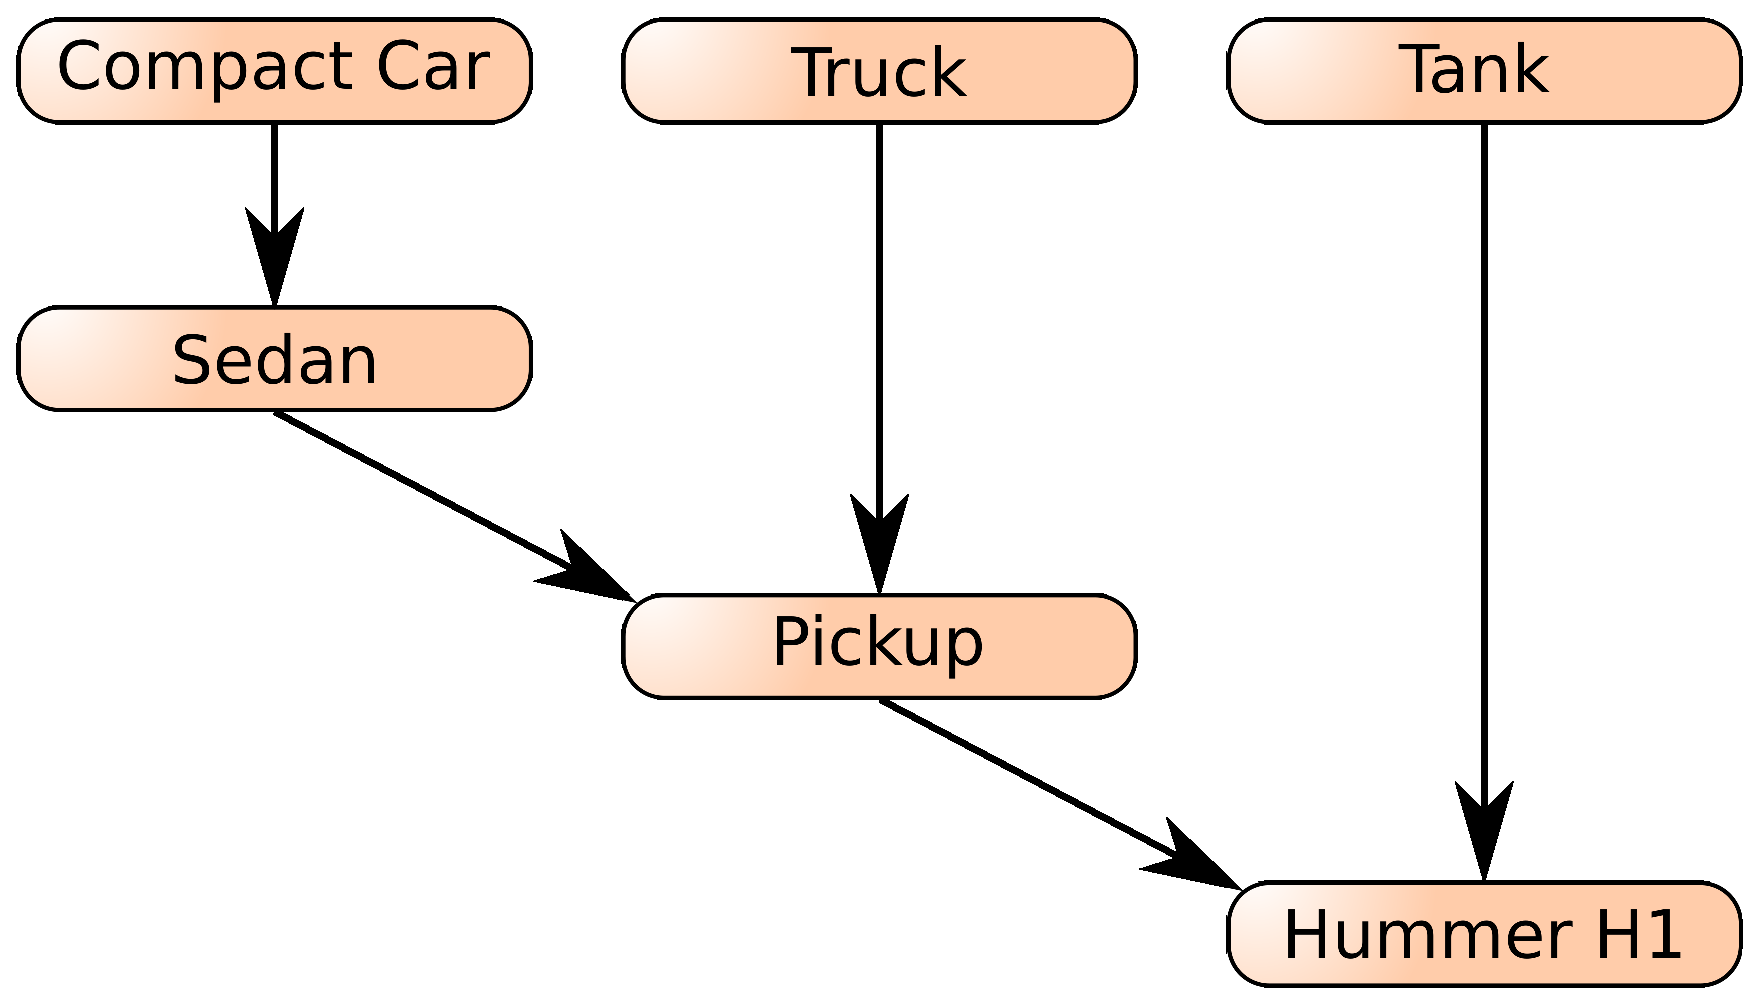
\includegraphics[width=.6\textwidth]{EPS/car-hierarchy.eps}
    \label{fig:car-hierarchy}
  }
  \subfloat[]{
    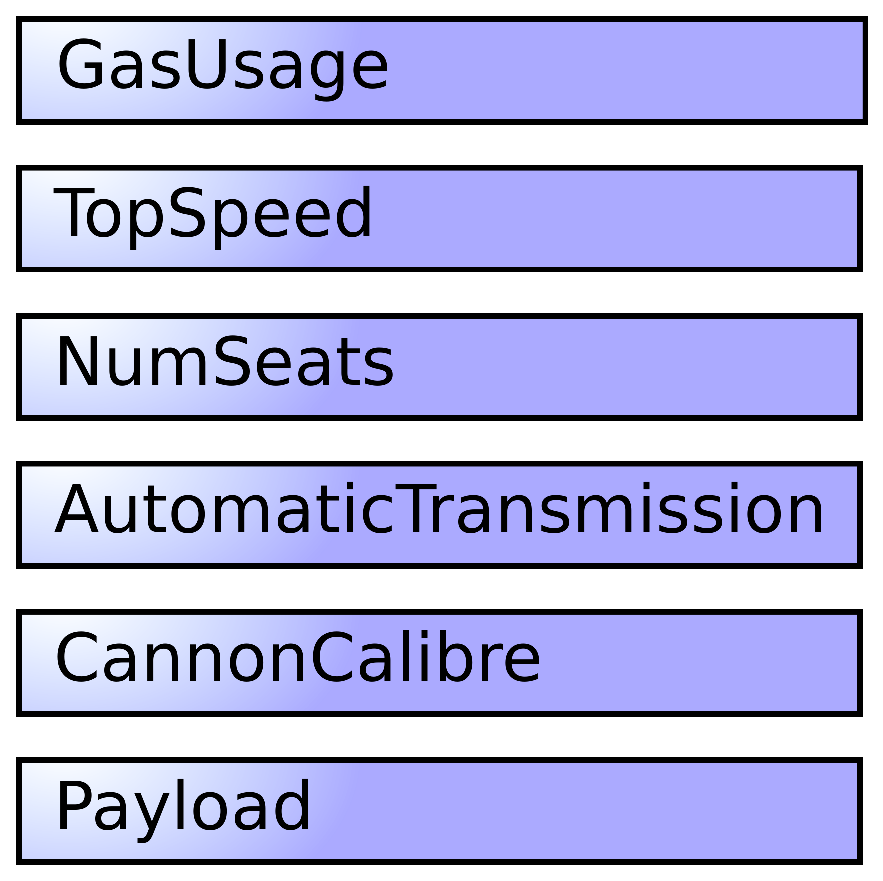
\includegraphics[width=.35\linewidth, keepaspectratio]{EPS/car-propertynames.eps}
    \label{fig:car-propertynames}
  }
  \caption{ \textbf{(a)}~~A possible property inheritance graph for
    various kinds of cars.  The lower nodes inherit from higher ones;
    Inherited properties from nodes on right take precedence over the
    properties defined on the left. ~~\textbf{(b)}~~Property names
    which make sense for at least one of the car types of (a).  }
\end{figure}

Using the \Dumux property system, this inheritance hierarchy is
defined by:
\begin{lstlisting}[name=propsyscars,basicstyle=\ttfamily\scriptsize,numbers=left,numberstyle=\tiny, numbersep=5pt]
#include <dumux/common/propertysystem.hh>
#include <iostream>

namespace Dumux {
namespace Properties {
NEW_TYPE_TAG(CompactCar);
NEW_TYPE_TAG(Truck);
NEW_TYPE_TAG(Tank);
NEW_TYPE_TAG(Sedan, INHERITS_FROM(CompactCar));
NEW_TYPE_TAG(Pickup, INHERITS_FROM(Sedan, Truck));
NEW_TYPE_TAG(HummerH1, INHERITS_FROM(Pickup, Tank));
\end{lstlisting}

Figure \ref{fig:car-propertynames} lists a few property names which
make sense for at least one of the nodes of Figure
\ref{fig:car-hierarchy}. These property names can be declared as
follows:
\begin{lstlisting}[name=propsyscars,basicstyle=\ttfamily\scriptsize,numbers=left,numberstyle=\tiny, numbersep=5pt]
NEW_PROP_TAG(TopSpeed); // [km/h]
NEW_PROP_TAG(NumSeats); // []
NEW_PROP_TAG(CanonCaliber); // [mm]
NEW_PROP_TAG(GasUsage); // [l/100km]
NEW_PROP_TAG(AutomaticTransmission); // true/false
NEW_PROP_TAG(Payload); // [t]
\end{lstlisting}

\noindent
So far, the inheritance hierarchy and the property names are completely
separate. What is missing is setting some values for the property
names on specific nodes of the inheritance hierarchy. Let us assume
the following:
\begin{itemize}
\item For a compact car, the top speed is the gas usage in $l/100km$
  times $30$, the number of seats is $5$ and the gas usage is
  $4\;l/100km$.
\item A truck is by law limited to $100\;km/h$ top speed, the number
  of seats is $2$, it uses $18\;l/100km$ and has a cargo payload of
  $35\;t$.
\item A tank exhibits a top speed of $60\;km/h$, uses $65\;l/100km$
  and features a $120\;mm$ diameter canon 
\item A sedan has a gas usage of $7\;l/100km$, as well as an automatic
  transmission, in every other aspect it is like for a compact car.
\item A pick-up truck has a top speed of $120\;km/h$ and a payload of
  $5\;t$. In every other aspect it is like sedan or a truck but if in
  doubt it is more like a truck.
\item The Hummer-H1 SUV exhibits the same top speed as a pick-up
  truck.  In all other aspects it is similar to a pickup and a tank,
  but if in doubt more like a tank.
\end{itemize}

\noindent
Using the \Dumux property system, these assumptions are formulated
using
\begin{lstlisting}[name=propsyscars,basicstyle=\ttfamily\scriptsize,numbers=left,numberstyle=\tiny, numbersep=5pt]
SET_INT_PROP(CompactCar, TopSpeed, GET_PROP_VALUE(TypeTag, PTAG(GasUsage)) * 30);
SET_INT_PROP(CompactCar, NumSeats, 5);
SET_INT_PROP(CompactCar, GasUsage, 4);

SET_INT_PROP(Truck, TopSpeed, 100);
SET_INT_PROP(Truck, NumSeats, 2);
SET_INT_PROP(Truck, GasUsage, 18);
SET_INT_PROP(Truck, Payload, 35);

SET_INT_PROP(Tank, TopSpeed, 60);
SET_INT_PROP(Tank, GasUsage, 65);
SET_INT_PROP(Tank, CanonCaliber, 120);

SET_INT_PROP(Sedan, GasUsage, 7);
SET_BOOL_PROP(Sedan, AutomaticTransmission, true);

SET_INT_PROP(Pickup, TopSpeed, 120);
SET_INT_PROP(Pickup, Payload, 5);

SET_INT_PROP(HummerH1, TopSpeed, GET_PROP_VALUE(TTAG(Pickup), PTAG(TopSpeed)));
\end{lstlisting}

\noindent
At this point, the Hummer-H1 has a $120\;mm$ canon which it inherited
from its military ancestor. It can be removed by
\begin{lstlisting}[name=propsyscars,basicstyle=\ttfamily\scriptsize,numbers=left,numberstyle=\tiny, numbersep=5pt]
UNSET_PROP(HummerH1, CanonCaliber);

}} // close namespaces
\end{lstlisting}

\noindent
Now property values can be retrieved and some diagnostic messages can
be generated. For example
\begin{lstlisting}[name=propsyscars,basicstyle=\ttfamily\scriptsize,numbers=left,numberstyle=\tiny, numbersep=5pt]
int main()
{
    std::cout << "top speed of sedan: " << GET_PROP_VALUE(TTAG(Sedan), PTAG(TopSpeed)) << "\n";
    std::cout << "top speed of truck: " << GET_PROP_VALUE(TTAG(Truck), PTAG(TopSpeed)) << "\n";

    std::cout << PROP_DIAGNOSTIC(TTAG(Sedan), PTAG(TopSpeed));
    std::cout << PROP_DIAGNOSTIC(TTAG(HummerH1), PTAG(CanonCaliber));
}
\end{lstlisting}
will yield the following output:
\begin{lstlisting}[basicstyle=\ttfamily\scriptsize,numbers=left,numberstyle=\tiny, numbersep=5pt]
top speed of sedan: 210
top speed of truck: 100
Property 'TopSpeed' for type tag 'Sedan'
  inherited from 'CompactCar'
    defined at test_propertysystem.cc:90
Property 'CanonCaliber' for type tag 'HummerH1'
  explicitly unset at test_propertysystem.cc:113
\end{lstlisting}


%%% Local Variables: 
%%% mode: latex
%%% TeX-master: "dumux-handbook"
%%% End: 
